% ============================================================
% LearnHub Internship Report - Chapters 1-5
% ============================================================
\documentclass[12pt,a4paper]{report}

\usepackage[utf8]{inputenc}
\usepackage[T1]{fontenc}
\usepackage{geometry}
\usepackage{graphicx}
\usepackage{hyperref}
\usepackage{listings}
\usepackage{xcolor}
\usepackage{titlesec}
\usepackage{fancyhdr}
\usepackage{tocloft}
\usepackage{booktabs}
\usepackage{array}
\usepackage{longtable}
\usepackage{enumitem}
\usepackage{caption}
\usepackage{float}
\usepackage{amsmath}
\usepackage{tikz}
\usetikzlibrary{shapes.geometric, arrows, positioning}

\geometry{margin=1in}
\hypersetup{colorlinks=true,linkcolor=blue,urlcolor=blue,citecolor=blue}

\definecolor{codebg}{RGB}{245,245,245}
\definecolor{codegreen}{RGB}{0,128,0}
\definecolor{codepurple}{RGB}{128,0,128}
\definecolor{codegray}{RGB}{128,128,128}

\lstdefinestyle{mystyle}{
    backgroundcolor=\color{codebg},
    commentstyle=\color{codegreen},
    keywordstyle=\color{codepurple}\bfseries,
    stringstyle=\color{red},
    basicstyle=\ttfamily\footnotesize,
    breaklines=true,
    frame=single,
    numbers=left,
    numberstyle=\tiny\color{codegray},
    tabsize=2,
    showstringspaces=false
}
\lstset{style=mystyle}

\pagestyle{fancy}
\fancyhf{}
\fancyhead[L]{\leftmark}
\fancyhead[R]{LearnHub -- E-Learning Platform}
\fancyfoot[C]{\thepage}

\titleformat{\chapter}[display]
  {\normalfont\huge\bfseries}{\chaptertitlename\ \thechapter}{20pt}{\Huge}

\begin{document}

% --- Title Page ---
\begin{titlepage}
\centering
\vspace*{1cm}
{\large \textbf{INTERNSHIP REPORT}\\[0.5cm]}
{\large on\\[0.5cm]}
{\Huge\bfseries LearnHub\\[0.3cm]E-Learning Platform\par}
\vspace{1cm}
{\Large\itshape A Full-Stack Web Application\par}
\vspace{1.5cm}
{\large
\begin{tabular}{rl}
\textbf{Technology Stack:} & MERN (MongoDB, Express, React, Node.js) \\
\textbf{Frontend:}         & React.js 18 with Vite 5 \\
\textbf{Backend:}          & Node.js / Express.js \\
\textbf{Database:}         & MongoDB (Mongoose ODM) \\
\textbf{Cloud Services:}   & Cloudinary CDN \\
\end{tabular}
\par}
\vspace{2cm}
{\large Submitted by: \textit{[Your Name Here]} \par}
\vspace{0.3cm}
{\large USN: \textit{[Your USN Here]} \par}
\vspace{0.3cm}
{\large Under the guidance of: \textit{[Guide Name Here]} \par}
\vspace{0.3cm}
{\large Organization: \textit{[Organization Name Here]} \par}
\vspace{1.5cm}
{\large Department of Computer Science and Engineering\\
\textit{[Your College Name Here]}\\[0.3cm]
\the\year\par}
\end{titlepage}

% --- Abstract ---
\chapter*{Abstract}
\addcontentsline{toc}{chapter}{Abstract}
This internship report documents the design, development, and deployment of \textbf{LearnHub}, a full-stack, role-based e-learning web application built during the internship period. LearnHub enables students to browse, purchase, and consume video-based courses while allowing instructors to create, manage, and monetize their educational content. The platform also includes an administrative dashboard for overseeing users, instructors, and courses. Key features include JWT-based authentication, OTP-driven password recovery, Cloudinary-hosted media, discussion forums, course progress tracking, and automated PDF certificate generation upon course completion. The application is built using the MERN stack (MongoDB, Express.js, React.js, Node.js) with Vite as the frontend build tool. This report covers the introduction, organization background, internship objectives, activities and tasks, learning experiences, outcomes, reflections, and conclusions drawn from the internship.

\tableofcontents
\listoffigures
\listoftables


% ============================================================
% CHAPTER 1 -- INTRODUCTION
% ============================================================
\chapter{Introduction}

\section{Background}
The rapid growth of online education has transformed the way knowledge is disseminated globally. E-learning platforms have become essential tools for both educators and learners, offering flexibility, accessibility, and scalability that traditional classroom settings cannot match. With the increasing demand for digital learning solutions, there is a significant need for robust, feature-rich platforms that can support the entire lifecycle of online education---from course creation and delivery to student engagement and certification.

\section{Purpose of the Internship}
The purpose of this internship was to gain practical, hands-on experience in full-stack web development by designing and building a production-ready e-learning platform from scratch. The internship provided an opportunity to apply theoretical knowledge of web technologies in a real-world project setting, working with modern tools and frameworks used in the software industry.

\section{Project Overview}
LearnHub is a modern, web-based e-learning platform designed to bridge the gap between instructors who wish to share knowledge and students who seek to acquire new skills. The platform operates as a three-role system comprising \textbf{Students}, \textbf{Instructors}, and an \textbf{Administrator}, each with distinct capabilities and dedicated interfaces.

The platform addresses key gaps in existing e-learning solutions by providing an integrated set of features including discussion forums, progress tracking, and automatic certificate generation within a single cohesive application.

\section{Technology Stack}
\begin{table}[H]
\centering
\caption{Technology Stack Summary}
\label{tab:techstack}
\begin{tabular}{@{}lll@{}}
\toprule
\textbf{Layer} & \textbf{Technology} & \textbf{Purpose} \\ \midrule
Frontend       & React 18 + Vite 5        & SPA UI framework \\
Styling        & Bootstrap 5, React-Bootstrap & Responsive design \\
Routing        & React Router DOM v6       & Client-side routing \\
HTTP Client    & Axios                     & API communication \\
Charts         & Chart.js + react-chartjs-2 & Earnings visualization \\
Icons          & React Icons               & UI iconography \\
Backend        & Node.js + Express 4       & REST API server \\
Database       & MongoDB + Mongoose 8      & NoSQL data storage \\
Authentication & JWT + bcryptjs            & Token-based auth \\
Email          & Nodemailer (Gmail SMTP)   & OTP and verification \\
File Storage   & Cloudinary + Multer       & Video/image hosting \\
PDF Generation & Puppeteer                 & Certificate creation \\
Deployment     & Vercel (vercel.json)      & Serverless deployment \\ \bottomrule
\end{tabular}
\end{table}

\section{Report Organization}
This report is organized into the following chapters:
\begin{enumerate}
    \item \textbf{Chapter 1 -- Introduction:} Background, purpose, and project overview.
    \item \textbf{Chapter 2 -- About the Organization:} Details about the internship organization.
    \item \textbf{Chapter 3 -- Objectives of Internship:} Goals and expected deliverables.
    \item \textbf{Chapter 4 -- Internship Activities and Tasks:} Detailed description of work performed.
    \item \textbf{Chapter 5 -- Learning Experiences:} Technologies and skills acquired.
    \item \textbf{Chapter 6 -- Learning Outcomes:} Measurable outcomes and competencies gained.
    \item \textbf{Chapter 7 -- Reflection and Analysis:} Critical analysis of the experience.
    \item \textbf{Chapter 8 -- Conclusion/Summary:} Summary and future scope.
    \item \textbf{Chapter 9 -- References:} Bibliography and resources used.
    \item \textbf{Chapter 10 -- Appendices:} Screenshots, code snippets, and supplementary material.
\end{enumerate}


% ============================================================
% CHAPTER 2 -- ABOUT THE ORGANIZATION
% ============================================================
\chapter{About the Organization}

\section{Organization Profile}
\textit{[Enter your organization/company name here]}

\textit{[Provide a brief description of the organization where the internship was carried out. Include details such as:]}
\begin{itemize}
    \item Name and location of the organization
    \item Year of establishment
    \item Industry sector (e.g., IT Services, EdTech, Software Development)
    \item Core business areas and services offered
    \item Number of employees and organizational scale
    \item Key clients or projects the organization has undertaken
\end{itemize}

\section{Vision and Mission}
\textit{[State the vision and mission of the organization.]}

\section{Products and Services}
\textit{[Describe the products, services, or solutions offered by the organization. If the organization specializes in web development, software consulting, or EdTech, detail these here.]}

\section{Work Environment}
During the internship, the work environment was collaborative and agile-oriented. The team followed modern software development practices including:
\begin{itemize}
    \item Version control using Git and GitHub
    \item Modular code architecture with separation of concerns
    \item RESTful API design principles
    \item Cloud-based media management using Cloudinary
    \item Environment-based configuration management using dotenv
\end{itemize}

\section{Role within the Organization}
As an intern, the primary role was that of a \textbf{Full-Stack Web Developer}, responsible for designing, developing, and testing both the frontend (React.js) and backend (Node.js/Express.js) components of the LearnHub e-learning platform.


% ============================================================
% CHAPTER 3 -- OBJECTIVES OF INTERNSHIP
% ============================================================
\chapter{Objectives of Internship}

\section{Primary Objectives}
The primary objectives of this internship were:
\begin{enumerate}[label=\arabic*.]
    \item To design and develop a fully functional, production-ready e-learning web application using the MERN stack.
    \item To implement secure, role-based authentication and authorization using JWT tokens and bcrypt password hashing.
    \item To build a comprehensive course management system allowing instructors to create, edit, and delete courses with multimedia content.
    \item To develop a student learning module with course browsing, purchasing, video consumption, progress tracking, and certificate generation.
    \item To create interactive discussion forums tied to individual courses for peer-to-peer learning.
    \item To build an administrative dashboard for platform-wide user, instructor, and course management.
    \item To integrate cloud-based media storage (Cloudinary) for scalable video and image hosting.
\end{enumerate}

\section{Secondary Objectives}
\begin{enumerate}[label=\arabic*.]
    \item To gain hands-on experience with modern frontend frameworks (React.js) and build tools (Vite).
    \item To learn backend API development using Express.js with MongoDB as the database.
    \item To understand and implement security best practices including password hashing, token-based authentication, and CORS configuration.
    \item To develop skills in integrating third-party services (Cloudinary, Nodemailer, Puppeteer).
    \item To practice responsive web design using Bootstrap 5 and React-Bootstrap.
    \item To understand the full software development lifecycle from requirements gathering to deployment.
\end{enumerate}

\section{Expected Deliverables}
\begin{itemize}
    \item A fully functional LearnHub web application with three user roles (Student, Instructor, Admin).
    \item RESTful API backend with 40+ endpoints covering authentication, courses, forums, and administration.
    \item Responsive frontend with 20+ pages/components.
    \item Database design with 5 MongoDB collections (User, Instructor, Course, Thread, OTP).
    \item Automated PDF certificate generation system.
    \item Project documentation and internship report.
\end{itemize}


% ============================================================
% CHAPTER 4 -- INTERNSHIP ACTIVITIES AND TASKS
% ============================================================
\chapter{Internship Activities and Tasks}

\section{Phase 1: Requirements Analysis and Planning}
The internship began with understanding the project requirements and planning the system architecture.
\begin{itemize}
    \item Studied existing e-learning platforms (Udemy, Coursera, edX) to identify key features and gaps.
    \item Defined three user roles: Student, Instructor, and Administrator with distinct capabilities.
    \item Created the system architecture following a three-tier client-server model.
    \item Selected the MERN stack based on JavaScript uniformity across the stack, community support, and scalability.
    \item Designed the database schema with five MongoDB collections.
\end{itemize}

\section{Phase 2: Backend Development}
\subsection{Server Setup and Configuration}
Set up the Express.js server with CORS, JSON body parsing, and MongoDB connection via Mongoose. The server mounts four route groups: \texttt{/users}, \texttt{/instructors}, \texttt{/admin}, and \texttt{/forums}.

\begin{lstlisting}[language=Java, caption={server.js -- Express Server Entry Point}]
const express = require('express');
const cors = require('cors');
require('dotenv').config();
const connectDB = require('./config/db');
const app = express();
app.use(cors({ origin: 'http://localhost:5173' }));
app.use(express.json());
connectDB();
app.use('/users', require('./routes/user'));
app.use('/instructors', require('./routes/instructor'));
app.use('/admin', require('./routes/admin'));
app.use('/forums', require('./routes/forum'));
const PORT = process.env.PORT || 5000;
app.listen(PORT, () => console.log(`Server on port ${PORT}`));
\end{lstlisting}

\subsection{Database Schema Design}
Designed five Mongoose models:

\begin{table}[H]
\centering
\caption{Database Collections Overview}
\begin{tabular}{@{}lp{8cm}@{}}
\toprule
\textbf{Collection} & \textbf{Key Fields} \\ \midrule
User & email, password (hashed), purchasedCourses[], coursesProgress[], name, username, linkedinUrl, githubUrl, phoneNumber, imageUrl \\
Instructor & email, password (hashed), name, username, linkedinUrl, githubUrl, phoneNumber, imageUrl \\
Course & title, price, description, imageUrl, requirements[], sections[\{title, description, videoUrl\}], instructorEmail \\
Thread & courseId, messages[\{userName, message, createdAt\}] \\
OTP & email, otp, expiresAt \\ \bottomrule
\end{tabular}
\end{table}

\subsection{Authentication System}
Implemented JWT-based authentication with:
\begin{itemize}
    \item User/Instructor registration with bcrypt password hashing (salt rounds: 10).
    \item Login endpoints returning signed JWT tokens (1-hour expiry).
    \item Auth middleware extracting and verifying tokens from \texttt{x-auth-token} header.
    \item Email verification via unique tokens.
    \item OTP-based password recovery using otp-generator and Nodemailer.
\end{itemize}

\subsection{API Development}
Developed 40+ RESTful API endpoints across four route files:

\begin{table}[H]
\centering
\caption{API Route Summary}
\begin{tabular}{@{}lcp{6cm}@{}}
\toprule
\textbf{Route Group} & \textbf{Endpoints} & \textbf{Key Functions} \\ \midrule
/users & 21 & Signup, login, OTP, profile CRUD, course purchase, progress tracking, certificate generation, search \\
/instructors & 18 & Signup, login, OTP, profile CRUD, course CRUD, video/image upload, enrolled students \\
/admin & 5 & List users/instructors/courses, delete courses, view instructor courses \\
/forums & 2 & Get thread messages, post new message \\ \bottomrule
\end{tabular}
\end{table}

\subsection{Utility Modules}
\begin{itemize}
    \item \textbf{Cloudinary (cloudinary.js):} Configured four Multer storage instances for course videos, course images, instructor profiles, and student profiles.
    \item \textbf{Certificate Generator (CertificateGenerator.js):} Uses Puppeteer to render styled HTML/CSS certificates with Google Fonts (Playfair Display, Great Vibes, Lora), gold accents, seal, and signature into downloadable PDFs.
    \item \textbf{Email (email.js):} Nodemailer transporter configured with Gmail SMTP for sending OTP emails.
\end{itemize}

\section{Phase 3: Frontend Development}
\subsection{Project Setup}
Initialized the React application using Vite with the following key dependencies: React 18, React Router DOM v6, Axios, Bootstrap 5, React-Bootstrap, Chart.js, and React Icons.

\subsection{Component Architecture}
Built 4 reusable components and 20+ page components organized by role:

\begin{table}[H]
\centering
\caption{Frontend Component Structure}
\begin{tabular}{@{}lp{8cm}@{}}
\toprule
\textbf{Category} & \textbf{Components} \\ \midrule
Shared Components & Header, HeaderStudent, Footer, SideBar \\
Student Pages (8) & Signup, Login, ForgotPassword, StudentDashboard, CourseDetails, Payment, CourseContent, StudentProfile \\
Instructor Pages (7) & InstructorAuth, InstructorDashboard, CreateCourse, EditCourse, Profile, EnrolledStudents, Earnings \\
Admin Pages (1) & Admin Dashboard \\
Navigation Pages (4) & ContactUs, Blog, Careers, TeacherGuidelines \\
Other (1) & LandingPage \\ \bottomrule
\end{tabular}
\end{table}

\subsection{Routing and Authentication}
Implemented client-side routing with protected routes using React Router's \texttt{Navigate} component. JWT tokens stored in localStorage with an Axios interceptor for automatic logout on 401 responses.

\subsection{Key Feature Implementations}
\begin{itemize}
    \item \textbf{Student Dashboard:} Three-tab interface (All Courses, My Courses, Discussion Forums) with course cards, progress bars, and threaded messaging.
    \item \textbf{Course Content Player:} Split layout with section sidebar (completion checkmarks), video player, ``Mark as Complete'' button, and certificate download at 100\% completion.
    \item \textbf{Instructor Dashboard:} Course management grid with sidebar navigation, course creation with video/image upload, and enrolled students view.
    \item \textbf{Admin Dashboard:} Tabular views for users, instructors, and courses with detail popups and delete actions.
    \item \textbf{Course Search:} Real-time search in HeaderStudent filtering courses by title, routing to course details or content based on purchase status.
\end{itemize}

\section{Phase 4: Testing and Debugging}
Performed comprehensive manual testing across all modules:

\begin{longtable}{@{}|c|p{2.8cm}|p{3cm}|p{2.5cm}|c|@{}}
\hline
\textbf{ID} & \textbf{Test Case} & \textbf{Input} & \textbf{Expected} & \textbf{Status} \\ \hline
\endhead
TC01 & Student Signup & Valid email + password & Account created & Pass \\ \hline
TC02 & Duplicate Signup & Existing email & Error 409 & Pass \\ \hline
TC03 & Student Login & Correct credentials & JWT returned & Pass \\ \hline
TC04 & Invalid Login & Wrong password & Error 400 & Pass \\ \hline
TC05 & Forgot Password & Valid email & OTP sent & Pass \\ \hline
TC06 & Course Creation & Valid data + media & Course saved & Pass \\ \hline
TC07 & Course Purchase & Auth user + courseId & Added to list & Pass \\ \hline
TC08 & Progress Tracking & Mark section done & Progress updated & Pass \\ \hline
TC09 & Certificate Gen & 100\% completion & PDF download & Pass \\ \hline
TC10 & Forum Post & Message text & Displayed & Pass \\ \hline
TC11 & Admin View & Admin access & All data listed & Pass \\ \hline
TC12 & Token Expiry & Expired JWT & Auto logout & Pass \\ \hline
\caption{Key Test Cases and Results}
\end{longtable}

\section{Phase 5: Deployment Preparation}
\begin{itemize}
    \item Configured \texttt{vercel.json} for serverless backend deployment.
    \item Set up environment variables for MongoDB URI, JWT secret, Cloudinary credentials, and email credentials.
    \item Organized project structure for production readiness.
\end{itemize}


% ============================================================
% LearnHub Internship Report - Chapters 5-10
% (Append after Chapter 4 content from Part 1)
% ============================================================


% ============================================================
% CHAPTER 5 -- LEARNING EXPERIENCES
% ============================================================
\chapter{Learning Experiences}

\section{Frontend Development with React.js}
Working on LearnHub provided extensive experience with React.js 18 and modern frontend development practices:
\begin{itemize}
    \item \textbf{Component-Based Architecture:} Learned to decompose complex UIs into reusable components (Header, HeaderStudent, Footer, SideBar) and role-specific page components organized in a modular directory structure.
    \item \textbf{React Hooks:} Gained proficiency with \texttt{useState} for state management, \texttt{useEffect} for side effects and API calls, and \texttt{useNavigate}/\texttt{useParams} from React Router for navigation.
    \item \textbf{Protected Routing:} Implemented authentication-guarded routes using React Router's \texttt{Navigate} component, conditionally rendering pages based on JWT token presence in localStorage.
    \item \textbf{Vite Build Tool:} Learned to use Vite for fast development server startup with Hot Module Replacement (HMR), environment variable management via \texttt{import.meta.env}, and optimized production builds.
\end{itemize}

\section{Backend Development with Node.js and Express.js}
The backend development phase provided deep understanding of server-side programming:
\begin{itemize}
    \item \textbf{RESTful API Design:} Designed and implemented 40+ API endpoints following REST conventions with proper HTTP methods (GET, POST, PUT, DELETE) and status codes.
    \item \textbf{Middleware Pattern:} Created and applied custom authentication middleware for route protection, and used third-party middleware (CORS, body-parser, Multer) for request processing.
    \item \textbf{Error Handling:} Implemented comprehensive error handling with try-catch blocks, appropriate HTTP status codes (400, 401, 403, 404, 409, 500), and meaningful error messages.
    \item \textbf{Environment Configuration:} Used dotenv for managing sensitive configuration (database URIs, API keys, secrets) separately from source code.
\end{itemize}

\section{Database Management with MongoDB}
\begin{itemize}
    \item \textbf{Schema Design:} Designed five interconnected Mongoose schemas with appropriate data types, required fields, unique constraints, and document references (ObjectId refs).
    \item \textbf{CRUD Operations:} Implemented full Create, Read, Update, and Delete operations using Mongoose methods (\texttt{find}, \texttt{findOne}, \texttt{findByIdAndUpdate}, \texttt{findByIdAndDelete}).
    \item \textbf{Data Relationships:} Managed document relationships using ObjectId references and the \texttt{populate()} method for joining related collections (e.g., User.purchasedCourses referencing Course).
    \item \textbf{Array Operations:} Used MongoDB operators like \texttt{\$addToSet} for preventing duplicate entries in arrays (purchased courses).
\end{itemize}

\section{Security Implementation}
\begin{itemize}
    \item \textbf{Password Hashing:} Learned to securely hash passwords using bcryptjs with salt rounds before storage, and compare hashed passwords during authentication.
    \item \textbf{JWT Authentication:} Implemented stateless authentication using JSON Web Tokens with configurable expiration, token verification middleware, and automatic session management.
    \item \textbf{OTP-Based Recovery:} Built a complete password recovery flow using one-time passwords with 10-minute expiration, generated via otp-generator and delivered via Nodemailer.
    \item \textbf{CORS Configuration:} Configured Cross-Origin Resource Sharing to restrict API access to the authorized frontend origin.
\end{itemize}

\section{Cloud Services and Third-Party Integration}
\begin{itemize}
    \item \textbf{Cloudinary CDN:} Integrated Cloudinary for scalable media storage with four separate upload configurations for course videos, course images, instructor profiles, and student profiles using Multer-Storage-Cloudinary.
    \item \textbf{Nodemailer:} Configured Gmail SMTP transport for sending verification emails and OTP codes.
    \item \textbf{Puppeteer:} Used headless Chrome automation to render professionally styled HTML/CSS certificates into downloadable PDF documents with custom fonts and graphics.
\end{itemize}

\section{UI/UX Design with Bootstrap}
\begin{itemize}
    \item Developed responsive layouts using Bootstrap 5's grid system, ensuring usability across desktop and mobile devices.
    \item Implemented interactive components using React-Bootstrap (Dropdowns, Cards, Modals, Progress Bars, Navigation Tabs).
    \item Created a collapsible sidebar for the instructor dashboard that auto-adjusts based on screen width.
    \item Built real-time course search with filtered dropdown results in the student header.
\end{itemize}


% ============================================================
% CHAPTER 6 -- LEARNING OUTCOMES
% ============================================================
\chapter{Learning Outcomes}

\section{Technical Competencies Acquired}

\begin{table}[H]
\centering
\caption{Technical Skills Gained During Internship}
\begin{tabular}{@{}clp{7cm}@{}}
\toprule
\textbf{No.} & \textbf{Skill Area} & \textbf{Competency Achieved} \\ \midrule
1 & React.js & Build complex SPAs with hooks, routing, protected routes, and state management \\
2 & Node.js/Express & Design and implement RESTful APIs with middleware, authentication, and error handling \\
3 & MongoDB/Mongoose & Design schemas, perform CRUD, manage references, and use aggregation \\
4 & JWT Authentication & Implement stateless, token-based auth with role-based access control \\
5 & Cloudinary & Integrate cloud media storage for videos and images with Multer \\
6 & Puppeteer & Generate styled PDF documents from HTML/CSS templates \\
7 & Git & Version control with branching, committing, and collaboration \\
8 & Bootstrap 5 & Build responsive, mobile-first user interfaces \\
9 & API Testing & Test endpoints manually and debug request/response cycles \\
10 & Deployment & Configure applications for Vercel serverless deployment \\ \bottomrule
\end{tabular}
\end{table}

\section{Software Engineering Practices}
\begin{enumerate}
    \item \textbf{Modular Architecture:} Learned to organize code into separate modules (models, routes, middleware, utils, components, pages) for maintainability and scalability.
    \item \textbf{Separation of Concerns:} Backend separates data models, business logic (routes), cross-cutting concerns (middleware), and utilities. Frontend separates reusable components from page-specific components.
    \item \textbf{Environment Management:} Used \texttt{.env} files for sensitive configuration, keeping secrets out of source code.
    \item \textbf{Error Handling Patterns:} Implemented consistent error handling with proper HTTP status codes and user-friendly error messages.
\end{enumerate}

\section{Project Deliverables Achieved}
\begin{itemize}
    \item[$\checkmark$] Fully functional three-role e-learning platform (Student, Instructor, Admin)
    \item[$\checkmark$] 40+ RESTful API endpoints with JWT authentication
    \item[$\checkmark$] 20+ responsive frontend pages/components
    \item[$\checkmark$] 5 MongoDB collections with proper relationships
    \item[$\checkmark$] Cloud-based media storage via Cloudinary
    \item[$\checkmark$] Automated PDF certificate generation
    \item[$\checkmark$] Course-specific discussion forums
    \item[$\checkmark$] Section-wise progress tracking with visual indicators
    \item[$\checkmark$] OTP-based password recovery system
    \item[$\checkmark$] Comprehensive project documentation
\end{itemize}


% ============================================================
% CHAPTER 7 -- REFLECTION AND ANALYSIS
% ============================================================
\chapter{Reflection and Analysis}

\section{Challenges Faced}

\subsection{Authentication Complexity}
Implementing dual authentication flows for students and instructors with separate registration, login, and profile management required careful API design to avoid route conflicts while maintaining code reusability.

\subsection{Media Upload Management}
Configuring Cloudinary with Multer for four different upload types (course videos, course images, instructor profiles, student profiles) required understanding of storage configurations, file type validation, and folder organization on the CDN.

\subsection{Progress Tracking Logic}
Designing the course progress tracking system with nested arrays in MongoDB (coursesProgress containing courseId, completedSections[], and lastSectionId) required careful handling of array updates and percentage calculations.

\subsection{Certificate Generation}
Rendering styled HTML with custom Google Fonts and complex CSS (diagonal corner accents, gold seals, signature images) into pixel-perfect PDFs using Puppeteer required extensive trial-and-error to achieve consistent output.

\subsection{Frontend State Management}
Managing authentication state across multiple routes, handling token expiration gracefully with Axios interceptors, and synchronizing localStorage with React state presented state management challenges.

\section{Solutions Implemented}
\begin{itemize}
    \item Organized routes into separate files (\texttt{user.js}, \texttt{instructor.js}) with distinct URL prefixes to avoid conflicts.
    \item Created a centralized \texttt{cloudinary.js} utility exporting four pre-configured Multer instances.
    \item Used MongoDB's \texttt{\$addToSet} operator and array manipulation methods for safe progress updates.
    \item Configured Puppeteer with explicit viewport dimensions and PDF page size matching the certificate design.
    \item Implemented an Axios response interceptor for centralized 401 handling with automatic token cleanup.
\end{itemize}

\section{Strengths of the Project}
\begin{enumerate}
    \item \textbf{Complete Feature Set:} Covers the full e-learning lifecycle from course creation to certificate issuance.
    \item \textbf{Role-Based Design:} Clean separation of Student, Instructor, and Admin functionalities.
    \item \textbf{Scalable Architecture:} Stateless JWT auth + Cloudinary CDN supports horizontal scaling.
    \item \textbf{Professional Certificates:} Auto-generated, beautifully styled PDF certificates add credibility.
    \item \textbf{Community Features:} Discussion forums promote peer-to-peer learning.
\end{enumerate}

\section{Areas for Improvement}
\begin{enumerate}
    \item Payment gateway integration (currently simulated) for real transactions.
    \item Implementing real-time features (WebSocket-based live chat, notifications).
    \item Adding quizzes and assessments for knowledge validation.
    \item Implementing course ratings and reviews.
    \item Adding comprehensive unit and integration testing.
\end{enumerate}

\section{Comparison with Existing Platforms}
\begin{table}[H]
\centering
\caption{Comparison with Existing E-Learning Platforms}
\begin{tabular}{@{}lcccc@{}}
\toprule
\textbf{Feature} & \textbf{Udemy} & \textbf{Coursera} & \textbf{edX} & \textbf{LearnHub} \\ \midrule
Video Courses        & Yes & Yes & Yes & Yes \\
Progress Tracking    & Yes & Yes & Yes & Yes \\
Certificates         & Paid & Paid & Paid & Free (Auto) \\
Discussion Forums    & Yes & Yes & Yes & Yes \\
Instructor Dashboard & Yes & Limited & Limited & Yes \\
Admin Panel          & Internal & Internal & Internal & Yes \\
Open Source          & No & No & No & Yes \\
Self-Hosted          & No & No & No & Yes \\ \bottomrule
\end{tabular}
\end{table}


% ============================================================
% CHAPTER 8 -- CONCLUSION/SUMMARY
% ============================================================
\chapter{Conclusion/Summary}

\section{Summary}
This internship provided a comprehensive, hands-on experience in full-stack web development through the design and implementation of LearnHub, a feature-rich e-learning platform. Over the course of the internship, the project progressed through all phases of the software development lifecycle---requirements analysis, system design, backend development, frontend development, testing, and deployment preparation.

LearnHub was successfully developed as a three-role platform supporting:
\begin{itemize}
    \item \textbf{Students:} Registration, course browsing, purchasing, video-based learning with progress tracking, discussion forums, and automated certificate generation.
    \item \textbf{Instructors:} Registration, course creation with video/image uploads to Cloudinary, course management (edit/delete), enrolled student tracking, and earnings analytics.
    \item \textbf{Administrators:} Platform oversight with user/instructor/course management and moderation capabilities.
\end{itemize}

\section{Key Achievements}
\begin{enumerate}
    \item Built a production-ready full-stack application using the MERN stack with 40+ API endpoints and 20+ frontend pages.
    \item Implemented secure authentication with JWT tokens, bcrypt hashing, and OTP-based password recovery.
    \item Integrated Cloudinary CDN for scalable media management across four content categories.
    \item Developed an automated certificate generation system using Puppeteer with professionally designed HTML/CSS templates.
    \item Created interactive discussion forums for community-driven learning.
    \item Achieved responsive design across all interfaces using Bootstrap 5.
\end{enumerate}

\section{Future Scope}
\begin{enumerate}
    \item \textbf{Payment Gateway:} Integrate Razorpay or Stripe for real payment processing.
    \item \textbf{Live Classes:} Add WebRTC-based live video sessions.
    \item \textbf{Quizzes:} Introduce section-wise assessments.
    \item \textbf{Ratings \& Reviews:} Enable course feedback from students.
    \item \textbf{Recommendation Engine:} ML-based course suggestions.
    \item \textbf{Mobile App:} React Native cross-platform application.
    \item \textbf{Multi-language:} Internationalization support.
    \item \textbf{Notifications:} Push and email notification system.
    \item \textbf{Analytics:} Advanced instructor analytics dashboards.
    \item \textbf{Content Moderation:} AI-based review for uploaded materials.
\end{enumerate}

\section{Personal Growth}
This internship significantly enhanced both technical and professional competencies. Working independently on a full-stack project developed problem-solving skills, time management, and the ability to learn new technologies rapidly. The experience of building a complete application from concept to deployment provided invaluable preparation for a career in software development.


% ============================================================
% CHAPTER 9 -- REFERENCES
% ============================================================
\chapter{References}

\begin{enumerate}[label={[\arabic*]}]
    \item React.js Documentation -- \url{https://react.dev/}
    \item Node.js Documentation -- \url{https://nodejs.org/en/docs}
    \item Express.js Documentation -- \url{https://expressjs.com/}
    \item MongoDB Documentation -- \url{https://www.mongodb.com/docs/}
    \item Mongoose Documentation -- \url{https://mongoosejs.com/docs/}
    \item Vite Documentation -- \url{https://vitejs.dev/}
    \item Cloudinary Documentation -- \url{https://cloudinary.com/documentation}
    \item JSON Web Tokens Introduction -- \url{https://jwt.io/introduction}
    \item Puppeteer Documentation -- \url{https://pptr.dev/}
    \item Bootstrap 5 Documentation -- \url{https://getbootstrap.com/docs/5.3/}
    \item React Router Documentation -- \url{https://reactrouter.com/en/main}
    \item Nodemailer Documentation -- \url{https://nodemailer.com/}
    \item Chart.js Documentation -- \url{https://www.chartjs.org/docs/latest/}
    \item Multer Documentation -- \url{https://github.com/expressjs/multer}
    \item bcrypt.js Documentation -- \url{https://github.com/dcodeIO/bcrypt.js}
    \item Axios Documentation -- \url{https://axios-http.com/docs/intro}
    \item React-Bootstrap Documentation -- \url{https://react-bootstrap.github.io/}
\end{enumerate}


% ============================================================
% CHAPTER 10 -- APPENDICES
% ============================================================
\chapter{Appendices (If Applicable)}

\section{Appendix A: Project Directory Structure}
\begin{lstlisting}[language={}, caption={Complete Project Structure}]
LearnHub/
|-- Client/                        # Frontend (React + Vite)
|   |-- src/
|   |   |-- Components/
|   |   |   |-- Header.jsx, HeaderStudent.jsx
|   |   |   |-- Footer.jsx, SideBar.jsx
|   |   |-- Pages/
|   |   |   |-- User/ (8 pages)
|   |   |   |-- Instructor/ (7 pages)
|   |   |   |-- Admin/ (1 page)
|   |   |   |-- Navs/ (4 pages)
|   |   |   |-- LandingPage.jsx
|   |   |-- App.jsx, main.jsx
|   |-- package.json, vite.config.js
|-- server/                        # Backend (Node + Express)
|   |-- config/db.js
|   |-- middleware/auth.js
|   |-- models/ (User, Instructor, Course, Thread, Otp)
|   |-- routes/ (user, instructor, admin, forum)
|   |-- utils/ (CertificateGenerator, cloudinary, email)
|   |-- server.js, package.json
|-- screenshots/                   # 16 application screenshots
\end{lstlisting}

\section{Appendix B: Application Screenshots}
\textit{Note: Uncomment the includegraphics lines and ensure screenshot files are accessible.}

\begin{enumerate}
    \item \textbf{Landing Page} -- Hero section, featured courses, categories, testimonials.
    % \begin{figure}[H]\centering\includegraphics[width=0.9\textwidth]{screenshots/Landing Page.png}\caption{Landing Page}\end{figure}

    \item \textbf{User Login} -- Student login form with email and password.
    % \begin{figure}[H]\centering\includegraphics[width=0.9\textwidth]{screenshots/User Login.png}\caption{User Login}\end{figure}

    \item \textbf{Student Dashboard} -- All Courses, My Courses, and Forums tabs.
    % \begin{figure}[H]\centering\includegraphics[width=0.9\textwidth]{screenshots/User Dashboard.png}\caption{Student Dashboard}\end{figure}

    \item \textbf{Course Details} -- Course info, instructor, requirements, enrollment.
    % \begin{figure}[H]\centering\includegraphics[width=0.9\textwidth]{screenshots/User Course Details.png}\caption{Course Details}\end{figure}

    \item \textbf{Course Content} -- Video player with section sidebar and progress.
    % \begin{figure}[H]\centering\includegraphics[width=0.9\textwidth]{screenshots/User Course Access.png}\caption{Course Content}\end{figure}

    \item \textbf{User Profile} -- Student profile management.
    % \begin{figure}[H]\centering\includegraphics[width=0.9\textwidth]{screenshots/User Profile.png}\caption{User Profile}\end{figure}

    \item \textbf{Discussion Forum} -- Course-specific threaded discussions.
    % \begin{figure}[H]\centering\includegraphics[width=0.9\textwidth]{screenshots/User Discussion.png}\caption{Discussion Forum}\end{figure}

    \item \textbf{Certificate} -- Auto-generated completion certificate.
    % \begin{figure}[H]\centering\includegraphics[width=0.9\textwidth]{screenshots/User Certificate.png}\caption{Certificate}\end{figure}

    \item \textbf{Instructor Login} -- Instructor authentication page.
    % \begin{figure}[H]\centering\includegraphics[width=0.9\textwidth]{screenshots/Instructor  Login.png}\caption{Instructor Login}\end{figure}

    \item \textbf{Instructor Dashboard} -- Course management with edit/delete.
    % \begin{figure}[H]\centering\includegraphics[width=0.9\textwidth]{screenshots/Instructor   Dashboard.png}\caption{Instructor Dashboard}\end{figure}

    \item \textbf{Course Creation} -- Multi-step course creation form.
    % \begin{figure}[H]\centering\includegraphics[width=0.9\textwidth]{screenshots/Instructor Course Creation.png}\caption{Course Creation}\end{figure}

    \item \textbf{Instructor Profile} -- Instructor profile management.
    % \begin{figure}[H]\centering\includegraphics[width=0.9\textwidth]{screenshots/Instructor Profile.png}\caption{Instructor Profile}\end{figure}

    \item \textbf{Enrolled Students} -- Students enrolled per course.
    % \begin{figure}[H]\centering\includegraphics[width=0.9\textwidth]{screenshots/Instructor Enrolled  Students.png}\caption{Enrolled Students}\end{figure}

    \item \textbf{Admin Dashboard} -- User, instructor, course management.
    % \begin{figure}[H]\centering\includegraphics[width=0.9\textwidth]{screenshots/Admin Dashboard 1.png}\caption{Admin Dashboard}\end{figure}
\end{enumerate}

\section{Appendix C: System Architecture Diagram}
\begin{figure}[H]
\centering
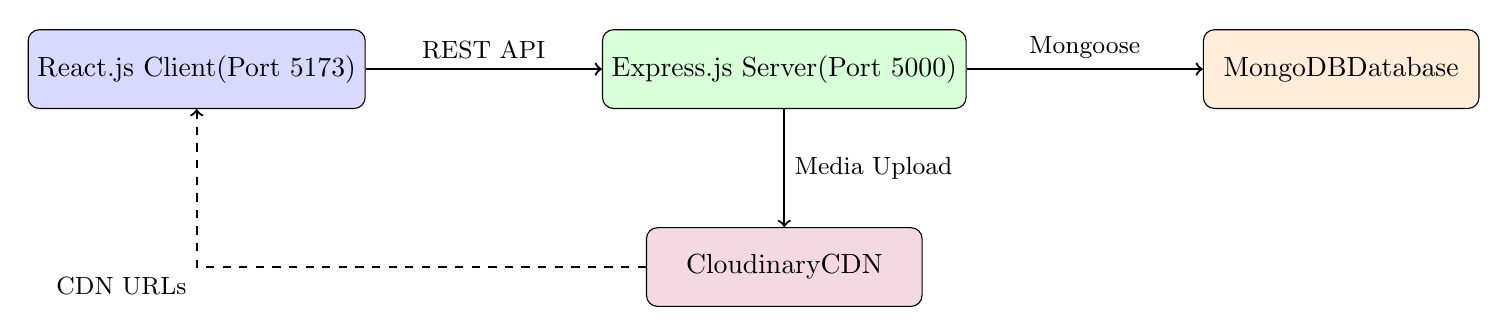
\begin{tikzpicture}[
    box/.style={rectangle, draw, minimum width=3.5cm, minimum height=1cm, text centered, rounded corners},
    arrow/.style={->, thick}
]
\node[box, fill=blue!15] (client) {React.js Client\\(Port 5173)};
\node[box, fill=green!15, right=3cm of client] (server) {Express.js Server\\(Port 5000)};
\node[box, fill=orange!15, right=3cm of server] (db) {MongoDB\\Database};
\node[box, fill=purple!15, below=1.5cm of server] (cloud) {Cloudinary\\CDN};

\draw[arrow] (client) -- node[above]{\small REST API} (server);
\draw[arrow] (server) -- node[above]{\small Mongoose} (db);
\draw[arrow] (server) -- node[right]{\small Media Upload} (cloud);
\draw[arrow, dashed] (cloud.west) -| node[below left]{\small CDN URLs} (client.south);
\end{tikzpicture}
\caption{System Architecture Diagram}
\label{fig:architecture}
\end{figure}

\section{Appendix D: Entity Relationship Diagram}
\begin{figure}[H]
\centering
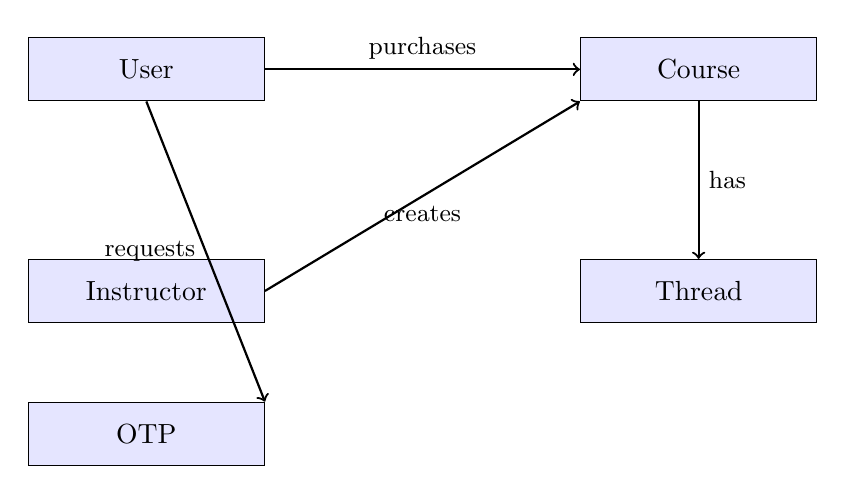
\begin{tikzpicture}[
    entity/.style={rectangle, draw, fill=blue!10, minimum width=3cm, minimum height=0.8cm, text centered},
    rel/.style={->, thick}
]
\node[entity] (user) {User};
\node[entity, right=4cm of user] (course) {Course};
\node[entity, below=2cm of user] (instructor) {Instructor};
\node[entity, below=2cm of course] (thread) {Thread};
\node[entity, below=1cm of instructor] (otp) {OTP};

\draw[rel] (user) -- node[above]{\small purchases} (course);
\draw[rel] (instructor.east) -- node[below]{\small creates} (course.south west);
\draw[rel] (course) -- node[right]{\small has} (thread);
\draw[rel] (user.south) -- node[left]{\small requests} (otp.north east);
\end{tikzpicture}
\caption{Entity Relationship Diagram}
\label{fig:erd}
\end{figure}

\section{Appendix E: Environment Variables}
\begin{lstlisting}[language={}, caption={Required Environment Variables (.env)}]
# Server (.env)
MONGODB_URI=mongodb+srv://<user>:<pass>@cluster.mongodb.net/learnhub
JWT_SECRET=<your-secret-key>
CLOUDINARY_CLOUD_NAME=<cloud-name>
CLOUDINARY_API_KEY=<api-key>
CLOUDINARY_API_SECRET=<api-secret>
EMAIL_USER=<gmail-address>
EMAIL_PASS=<gmail-app-password>
PORT=5000

# Client (.env.local)
VITE_REACT_APP_BACKEND_BASEURL=http://localhost:5000
\end{lstlisting}

\end{document}
